% !TeX spellcheck = en_GB
% Chapter 1

\chapter{A Review of NeuCube: An Evolving Spatio-Temporal Data Machine Framework} % Main chapter title

\label{chap:neucube} % For referencing the chapter elsewhere, use \ref{Chapter1} 

%----------------------------------------------------------------------------------------

% Define some commands to keep the formatting separated from the content 
In the last decade or so, with the advent of deep neural network, a significant proportion of research in artificial intelligence and machine learning has been conducted in the area of neural networks. This has led to a massive diversification in the architecture and functionality of the neural networks. This diversity across the domain of neural networks makes it extremely difficult to review the area exhaustively or even perform systematic taxonomy as such. \citet{neuralnetworkzoo} has visually demonstrated (see \figurename \ref{fig:neural_network_archs}) the node level block architectures of several popular neural networks. This is a very useful comparative diagram to provide broad understanding of different neural networks. However, care must be taken in interpreting the networks from the figure as the node level diagram hides several degrees of abstractions and similar looking architectures (e.g. VAE and DAE), which may be greatly different with respect to training protocol and application areas. 
\begin{figure}
	\centering
	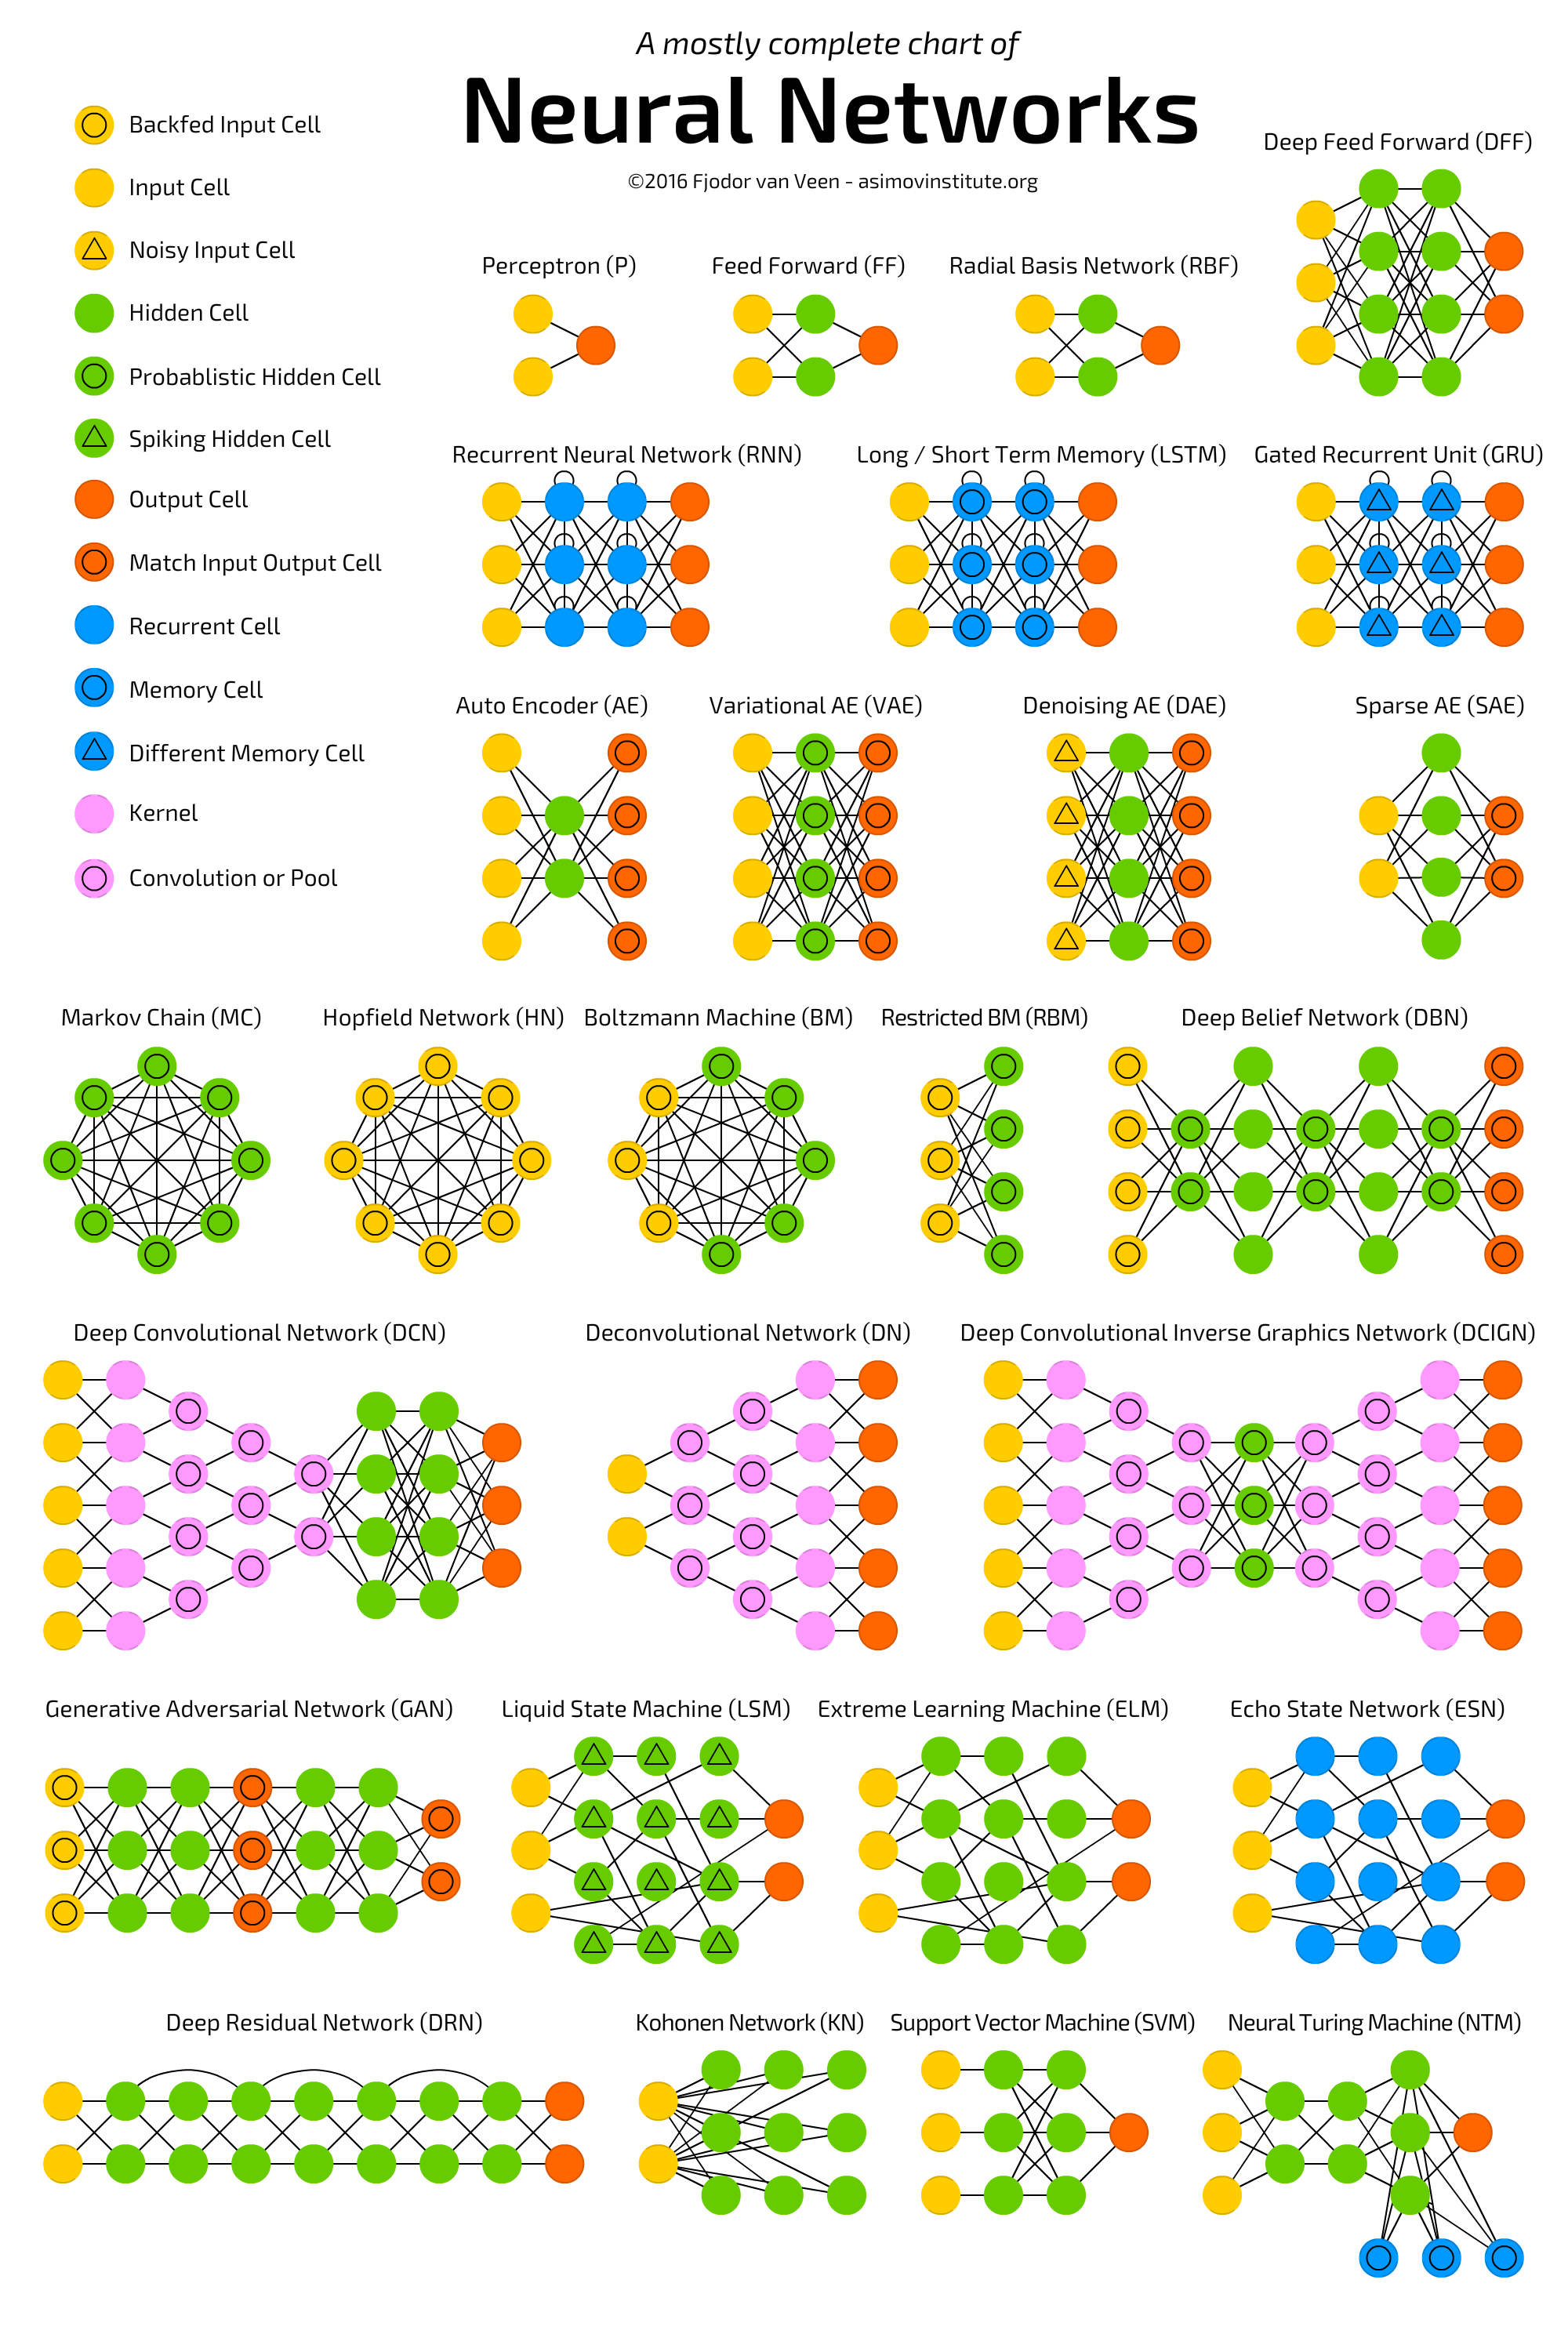
\includegraphics[width=0.8\linewidth]{fig/neucube/arch_comp.png}
	\caption{Node level architectures of popular neural networks (source \citet{neuralnetworkzoo}).}
	\label{fig:neural_network_archs}
\end{figure}

In this Chapter, the focus will be shifted towards discussing the novel evolving spatio-temporal data machine, NeuCube, proposed by Nikola Kasabov in \citep{kasabov2012neucube}. This framework is especially designed to take advantage of heterogeneous properties present in the data, especially in the form of spatial and temporal information. NeuCube draws its inspiration from the of recurrent neural network based reservoir computing paradigm and this topic will be discussed further. 

\section{Recurrent Neural Networks}

Rather than diverting into describing all the networks (see \citep{neuralnetworkzoo} for a brief description of all the architectures shown in \figurename \ref{fig:neural_network_archs}), I will concentrate on the recurrent neural networks (RNN). RNNs can be described simply as feed forward neural networks (FFNN) with a time twist. RNNs consist of a set of processing elements (neurons) which are interconnected by abstractions of synaptic connections. The interconnected mesh enables activations to be propagated through the network. The characteristic feature that differentiates RNN from FFNN is the connection topology. RNNs possess cyclic connections forming intra and inter-layer loops. The existence of cyclic connection has profound impact: 
\begin{enumerate}
	\item Even in the absence of input signals, RNNs possess the ability to develop a self-sustained activation dynamics along the cyclic connections. This property allows RNNs to act as a dynamic system as opposed to the function like behaviour of FFNN.
	\item RNNs possess dynamic memory and are able to make use of temporal contextual information. 
\end{enumerate}

The philosophy of the recurrent neural network is rooted in the fact that humans do not start thinking from scratch every second. When an individual reads or speaks, their understanding of a concept at any point in time is contextually dependent on what they understood earlier. Thoughts have persistence. Traditional neural networks are not capable of using information in a contextual manner, which is a major shortcoming. For example, to classify events in a video over time, it is unclear how a traditional neural network could use its reasoning about previous events in the video to inform future events.

RNNs are built to address this exact issue. The network retains information by including loops in them. On the left hand side of \figurename \ref{fig:rnn_unrolled}, a RNN block is shown. Block $A$, receives some input $x_t$ and outputs a value $h_t$. A loop passes the information from one step of the network to the next step \citep{rnnexplanation}. An RNN can be intuitively described as multiple copies of the same network unrolled across the time dimension (see \figurename \ref{fig:rnn_unrolled}). This chain-like nature reveals that recurrent neural networks are intimately related to sequences and lists. They are the natural architecture of neural networks to use for such data.

\begin{figure}
	\centering
	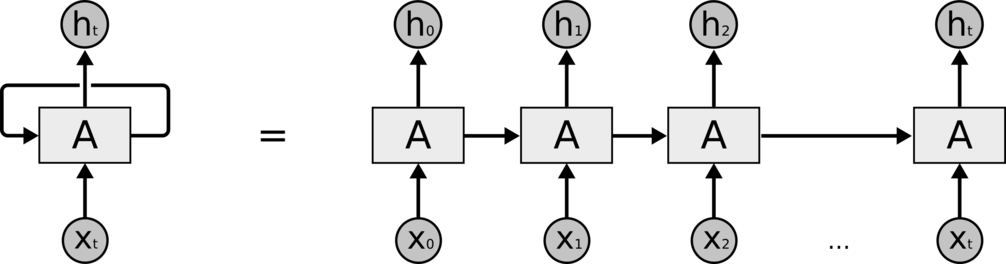
\includegraphics[width=.7\linewidth]{fig/neucube/RNN-unrolled.png}
	\caption{Unrolled RNN (source \citet{rnnexplanation}).}
	\label{fig:rnn_unrolled}
\end{figure}

\subsection{What Makes RNN Effective?}
\begin{figure}
	\centering
	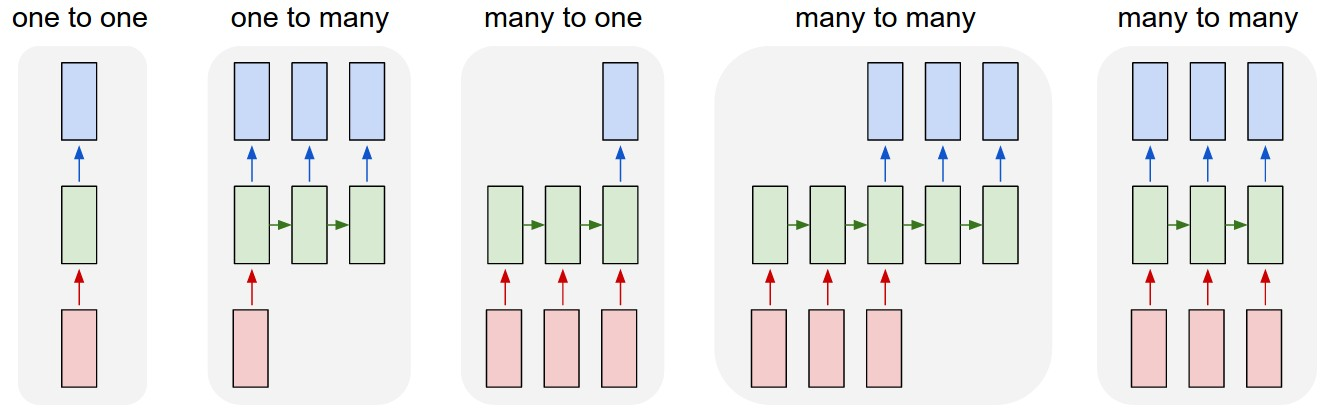
\includegraphics[width=.7\linewidth]{fig/neucube/rnn_karpathy.jpeg}
	\caption{Mapping capabilities of RNN (source \citet{effectivernn}).}
	\label{fig:rnn_karpathy}
\end{figure}
Andrej Karpathy in his blog post \citep{effectivernn} addresses this question with great detail. In his post, he argued that the ability of the RNNs to operate over sequences of vectors, input, output or both makes it more powerful. \figurename \ref{fig:rnn_karpathy} taken from \citep{effectivernn} describes the effectiveness with respect to mapping capabilities of RNN. Each rectangle in the figure represents a vector and the arrows are functions (such as matrix multiplication). The input vectors are coloured in red, output vectors in blue and RNN hidden states in green. From left to right, it shows: (1) The typical FFNN style vanilla processing with fixed size input and output; (2) Sequence of outputs (Image captioning. One image as input and a sequence of words as output); (3) Sequence of inputs (Sentiment analysis. Sequence of word as input and sentiment as output); (4)Sequence input and delayed sequence output (Machine translation); and, (5)  Synced sequence input and output (Video frame labelling).

From a dynamic system viewpoint, two major classes of RNNs exist. The first class of models are characterised by symmetric connections and energy minimising stochastic dynamics \citep{lukovsevivcius2009reservoir}. The best known architectures of this category are Hopfield Network \citep{hopfield1982neural}, Boltzmann Machine \citep{hinton1986learning}, Deep Belief Network \citep{bengio2007greedy} and Long Short Term memory \citep{hochreiter1997long}. These networks are mostly trained in some unsupervised learning scheme. Typical targeted network functionalities in this field are associative memories, data compression, the unsupervised modelling of data distributions, and static pattern classification, where the model is run for multiple time steps per single input instance to reach some type of convergence. In contrast, the second big class of RNN models typically features a deterministic update dynamics and directed connections. Systems from this class implement non-linear filters, which transform an input time series into an output time series. The mathematical background here is non-linear dynamical systems \citep{lukovsevivcius2009reservoir}. I will focus on the second category of RNNs as part of my work.

\section{Formalisation of the Temporal Learning Problem}
A traditional machine learning task can be expressed mathematically as the learning of functional dependence given an input $x(n)\in \mathbb{R}^{N_x}$ and ground truth $y(n) \in \mathbb{R^{N_y}}$, where $n=1,\cdots, T$, and $T$ is the number of samples in the training dataset $\{x(n), y(n)\}$. In a static data scenario, there is no temporal dependence between the samples, and the objective is to learn a function $\hat{y}= f(x)$, such that the error or loss function $E(\hat{y}, y)$ is minimised. On the contrary, in a temporal task, $x$ and $y$ are signals in a discrete time domain $n=1,\cdots, T$, and the goal is to learn $\hat{y}=f(x(1),\cdots,x(n-1), x(n))$, such that that $E(\hat{y}, y)$ is minimised. This formalism clearly shows that in the temporal learning scenario, the function learned is stateful or memory driven as opposed to the stateless non-temporal task. In a dynamic filter approach of RNN, it typically implements the non-linear expansion of memory as a state vector of the form described in the equation below:

\begin{equation}
	h(n)=f(W_{in}x(n)+Wx(n-1),\cdots), \ n=1, \cdots, T
\end{equation}

where $h$ is the activation function of a computational unit.

\section{Reservoir Computing and Liquid State Machines}
\begin{figure}
	\centering
	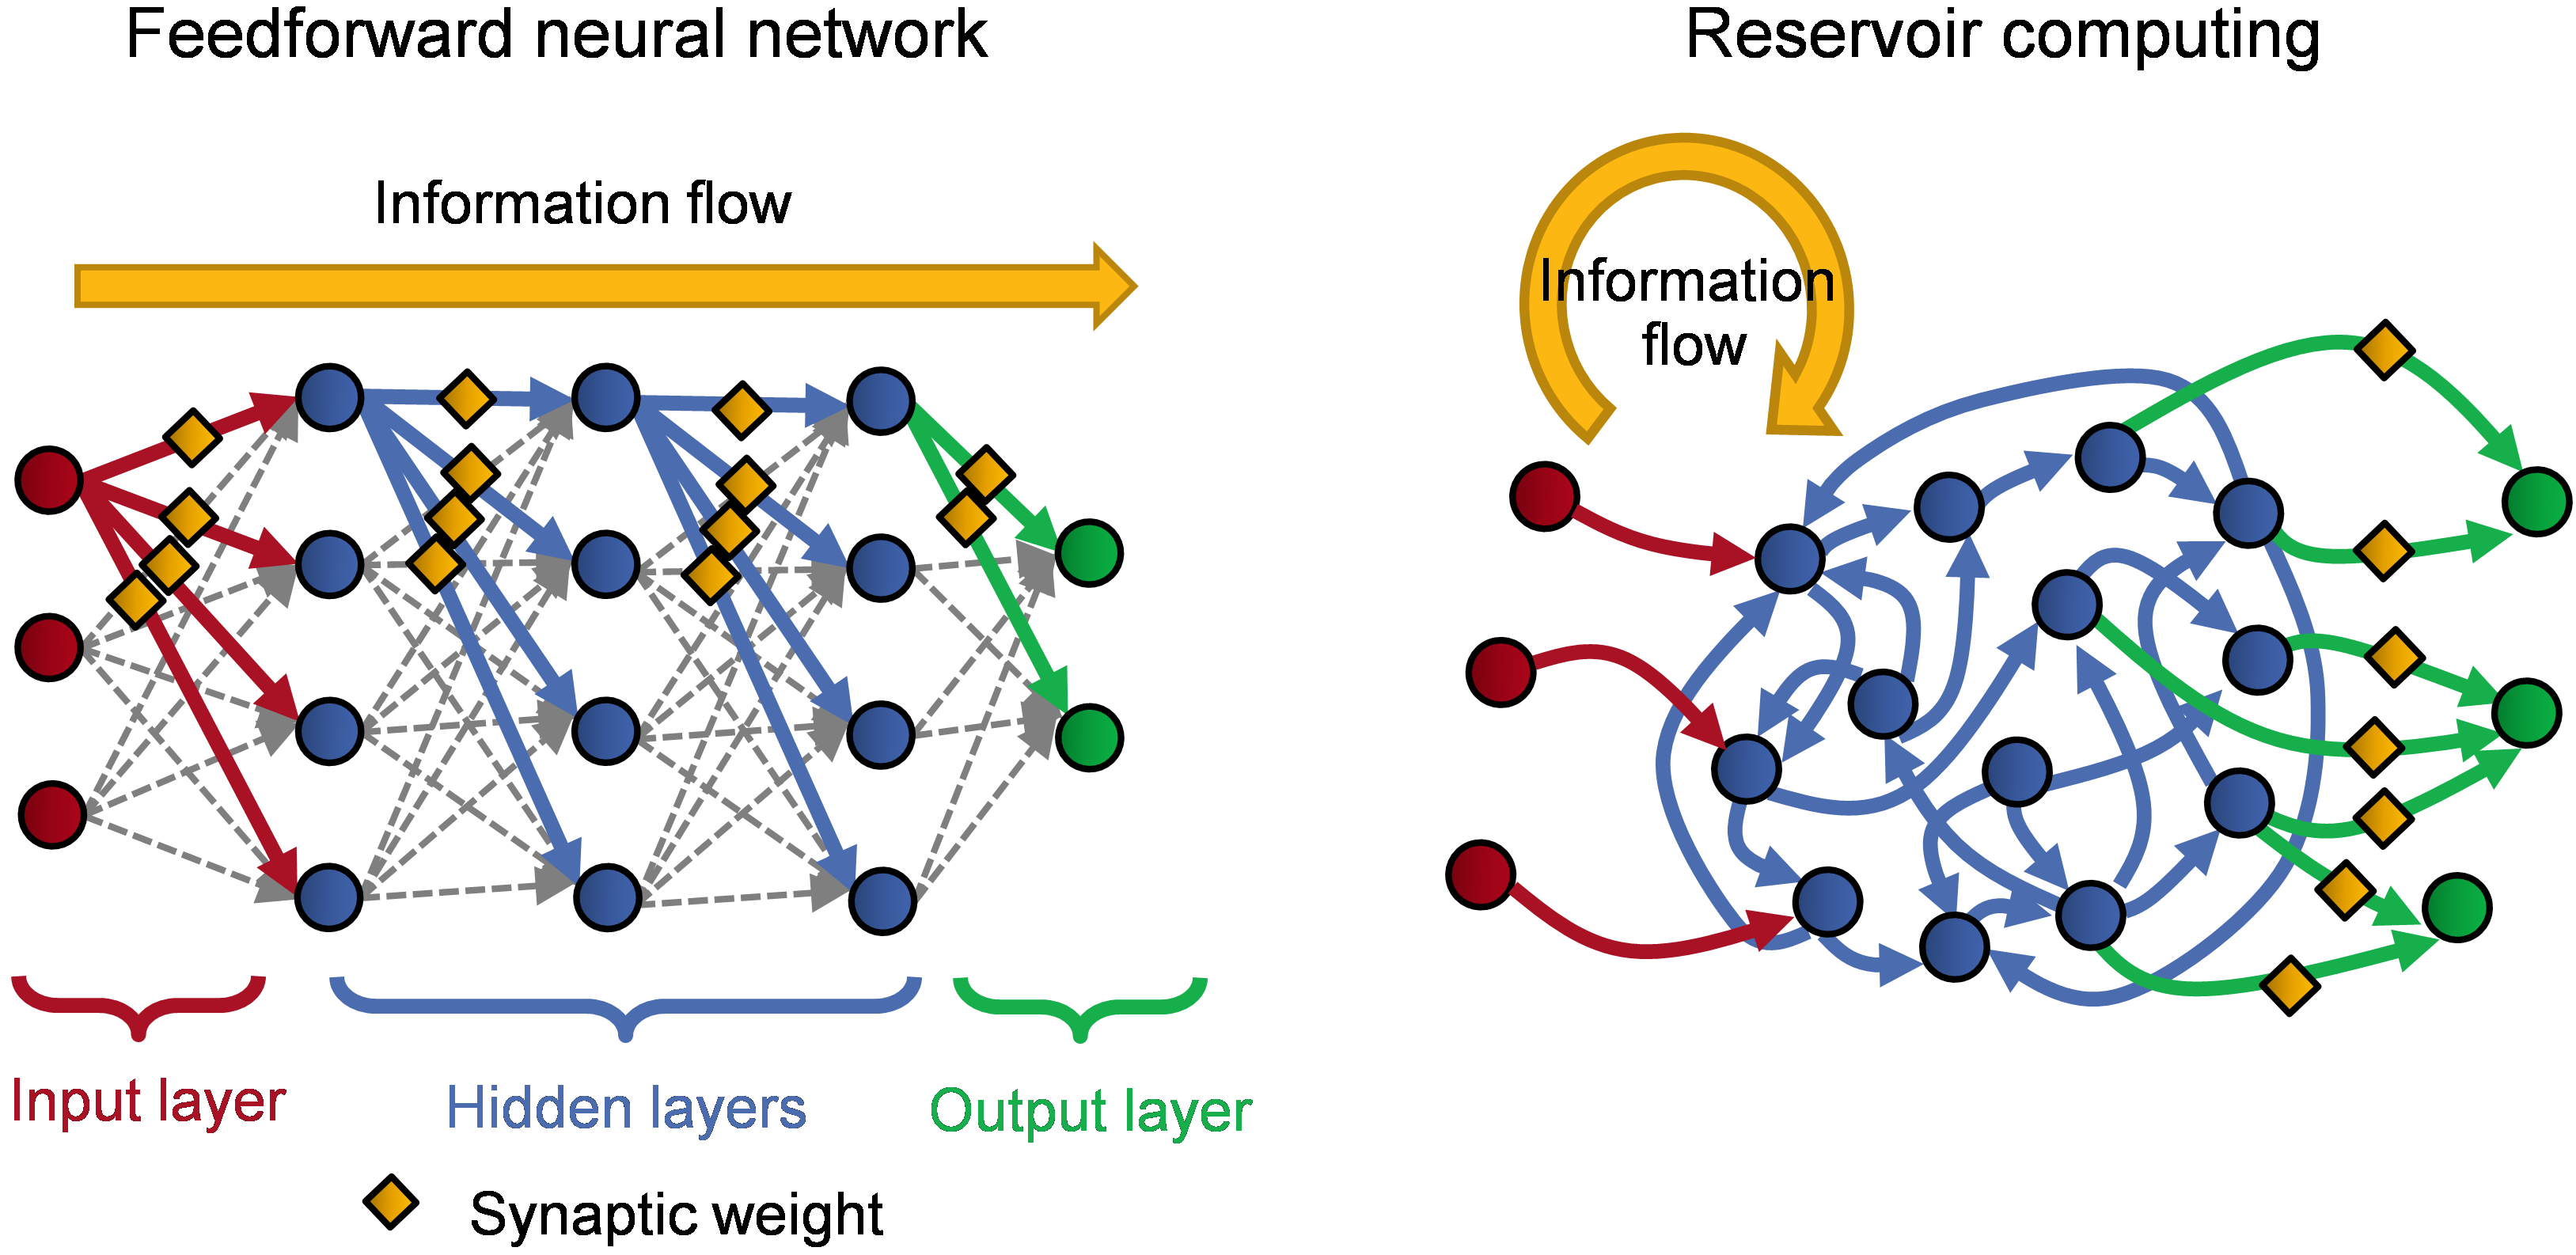
\includegraphics[scale=0.1]{fig/neucube/reservoir.png}
	\caption{Schematic diagram of a feed forward neural network vs. a reservoir computing system (source \citet{ibm2018stefan}).}
	\label{fig:reservoir_feedforward}
\end{figure}

\figurename \ref{fig:reservoir_feedforward} compares the node level diagram of a typical FFNN and the reservoir computing approach. Reservoir computing as described by \citet{schrauwen2007overview} is a dynamic filter, where an input signal is fed into a fixed and random dynamic system called reservoir, and the dynamics of the reservoir performs non-linear expansion of the input into a higher dimensional space. A recurrence-free readout mechanism then takes the data and maps it to the desired output. \figurename \ref{fig:reservoir_intuition} shows the intuition of reservoir computing paradigm in a schematic diagram. Since the expansion and the readout serve different purposes, training/generating them separately and even with different goal functions makes sense. The blue nodes in FFNN acts as non-dynamic and non-linear transfer functions. 	On the other hand, the blue nodes in a reservoir computing paradigm acts as a reservoir of recurrently connected neurons which possess the ability to act stateful and transform data into a higher dimensional space for the readout layer (green) to map into output with relative ease. The "traditional" RNN training methods do not make the conceptual separation of a reservoir vs. a readout, and train both reservoir-internal and output weights in technically the same fashion. For a detailed review of reservoir computing, see \citep{lukovsevivcius2009reservoir}.
\begin{figure}
	\centering
	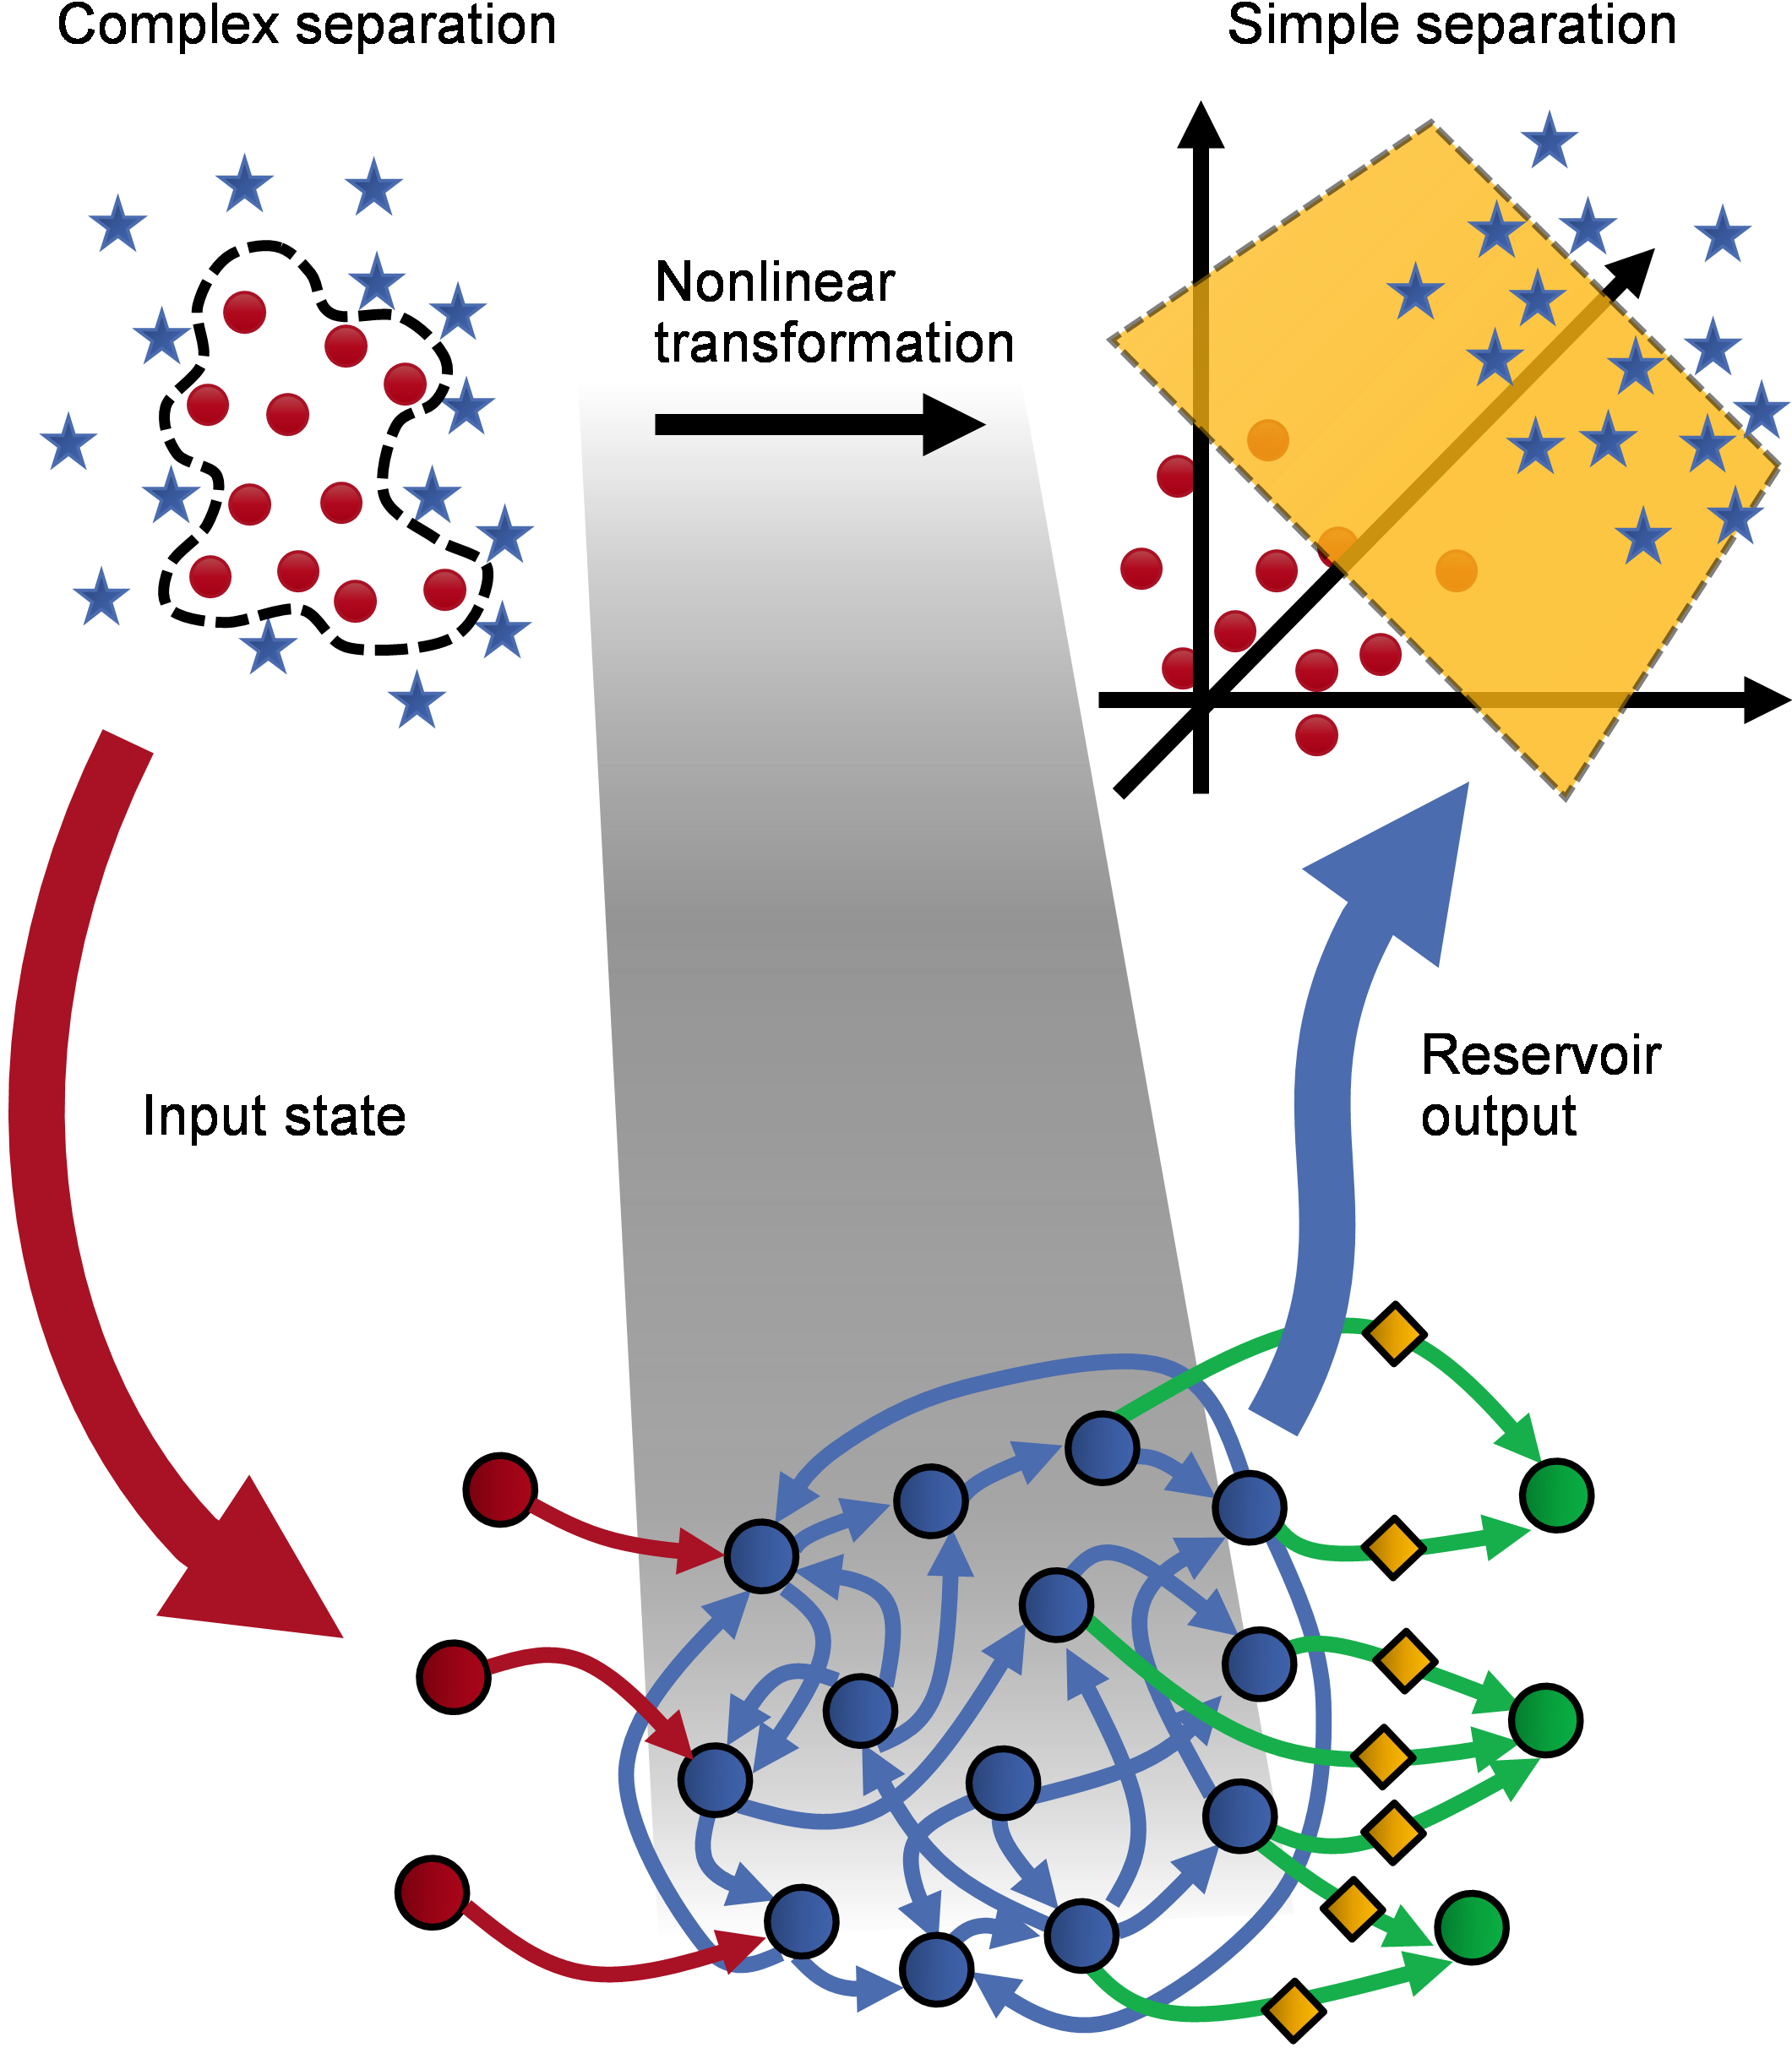
\includegraphics[scale=0.1]{fig/neucube/reservoir_intuition.png}
	\caption{Principle of reservoir computing: The input states are transformed into a high-dimensional feature space where classification can be performed with linear operation (source \citet{ibm2018stefan}).}
	\label{fig:reservoir_intuition}
\end{figure}

\subsection{Liquid State Machines}


Liquid State Machines (LSM) are a special kind of RNN architecture within the reservoir computing paradigm proposed by \citet{maass2002real}. LSMs were primarily intended for elucidating computational properties of microcircuits from a computational neuroscience perspective. Therefore, LSMs  possess great sophistication and biological realism  with respect to the behaviour of the neurons within the reservoir. The reservoir of LSM is often described as a liquid state. Input data feeds to the reservoir resembles "throwing pebbles into a pond" creating ripples in the fluid in the reservoir. The interaction of the ripples creates useful patterns over space and time. The neurons of LSM are spiking in nature and due to the biological plausibility are extremely complex and parameter-heavy in nature. For this reason, the LSMs have proven to be not only computationally expensive but also difficult to tune. However, a major advantage of using LSM is its ability to perform complex information processing through temporal encoding in a highly efficient manner. I will provide discussion on this topic in Chapter \ref{chap:encoding}. The main theoretical contributions of the LSM brand to reservoir computing consist in analytical characterisations of the computational power of such systems.  

\section{NeuCube Evolving Spatio-temporal Data Machine}
\label{sec:neucube_estdm}
The brain is a complex integrated spatio-temporal information processing machine. The mammalian brain is made up of spatially distributed structural and functional areas constrained within a three dimensional space. External stimuli and/or inner processes are of a varying nature, such as visual, auditory, somatosensory, olfactory and so on, from which emanate a complex spatio-temporal activity path within the brain leading to highly efficient and accurate recognition of patterns.

For example \citet{benuskova2010computational} provide the following example:

"$\cdots$ the language task involves transfer of information from
the inner ear through the auditory nucleus in thalamus to the primary auditory cortex (Brodmann’s area 41), then to the higher-order auditory cortex (area 42), before it is relayed to the angular gyrus (area 39). Angular gyrus is a specific region of the parietal-temporal-occipital association cortex, which is thought to be concerned with the association of incoming auditory, visual and tactile information. From here, the information is projected to Wernicke’s area (area 22) and then, by means of the arcuate fasciculus, to Broca’s area (44, 45), where the perception of language is translated into the grammatical structure of a phrase and where the memory for word articulation is stored. This information about the sound pattern of the phrase is then relayed to the facial area of the motor cortex that controls articulation so that the word can be spoken. It turns out that a similar pathway is involved in naming an object that has been visually recognised. This time, the input proceeds from the retina and LGN (lateral geniculate nucleus) to the primary visual cortex, then to area 18, before it arrives at the angular gyrus, from where it is relayed by a particular component of arcuate fasciculus directly to Broca’s area, bypassing Wernicke’s area." 

The example above shows that the brain processes information through the activation of complex spatiotemporal trajectories involving multiple functional areas. The NeuCube evolving Spatio-Temporal Data Machines are derived exactly from this very philosophy.

\begin{figure}
	\centering
	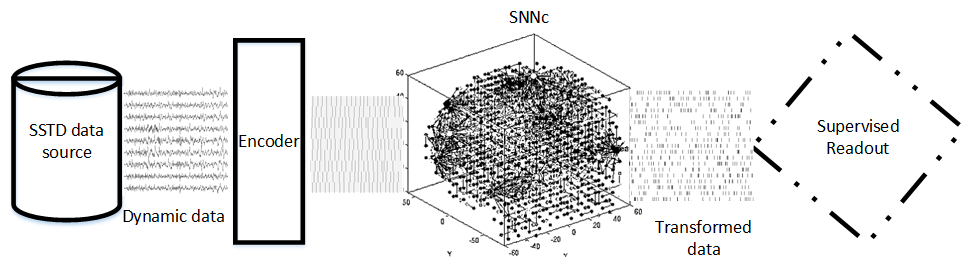
\includegraphics[width=\linewidth]{fig/neucube/neucube_arch.png}
	\caption{Schematic architecture diagram of NeuCube.}
	\label{fig:neucube_archit}
\end{figure}

The generic principles of the NeuCube architecture was introduced in \citep{kasabov2012neucube} and was further elaborated in \citep{kasabov2014evolving, kasabov2017mapping, sengupta2018from}. \figurename \ref{fig:neucube_archit} shows a schematic diagram of the NeuCube evolving Spatio-Temporal Data Machine (eSTDM) architecture. This framework is designed to use the spatial and temporal relationships in the data and therefore expects a spatio-temporal data source to feed spatio or spectro temporal data (SSTD) to the system. The NeuCube framework is a tiered architecture of three layers.
\subsection{Encoding}
The encoding layer is the first layer of NeuCube. This layer is responsible for converting real world continuous SSTD into a sequence of events or binary spikes. Formally, the encoding layer transforms real continuous data $\mathbb{R}^{N\times T}$ ($N$ is the feature count or the spatial component and $T$ is the temporal component) into spike trains $\lbrace 0,1 \rbrace^{N\times T}$. Numerous temporal encoding algorithms like BSA \citep{schrauwen2003bsa}, temporal contrast, GAGamma  \citep{sengupta2015framework} are proposed and used in an application specific manner. The data encoding layer in NeuCube can also be observed as a data compression layer which has the unique property of compressing data in temporal domain by representing important events by spike-timings. In the temporal encoding scheme, the timings of the spikes are considered to be useful rather than the quantity of the spike. This is  in contrast to the traditional data compression algorithms like auto-encoder and PCA, as the compression in the data is performed in a temporal dimension of the data. \citet{sengupta2017spike} discusses the temporal encoding by spike-time representation in the light of data compression and information theory, and compares the capabilities of different temporal encoding algorithms. 

\subsection{SNNc}
The SNNc layer is claimed to be the most complex and novel component of this architecture. It is an unsupervised learning layer composed of a 3D grid of spatially arranged spiking and input neurons. Each neuron inside the grid has a spatial location and resides within a neighbourhood of other neurons. This grid is known as the spiking neural network cube (SNNc) in the NeuCube architecture. The purpose of the SNNc layer is to transform the compressed spike representation of input data into a higher-dimensional space through unsupervised learning ($g:\lbrace 0,1 \rbrace^{N \times T}\rightarrow \lbrace 0, 1 \rbrace^{M \times T}| M>>N$) inside an SNNc, using a modified Hebbian spike-time dependent plasticity (STDP) learning \citep{song2000competitive}. The purpose of learning in the SNNc is to dynamically update the synaptic strengths within the network to mimic spatio-temporal synchronicity in the data. 

\subsubsection{STDP Learning}

STDP is a temporally asymmetric form of Hebbian learning induced by temporal correlations between the spikes generated by the pre and post-synaptic neurons. With STDP, repeated pre-synaptic spike arrival earlier than post-synaptic spike release leads to strengthening of the synapse known as long-term potentiation (LTP), and, in contrast, repeated spike arrival after post-synaptic spikes leads to weakening of the synapses known as long-term depression (LTD). The change of the synapse plotted as a function of the relative timing of pre- and post-synaptic action potentials is called the STDP function or learning window and varies between synapse types. I will formalise and discuss on the STDP learning rule and its variations as part of Chapter \ref{chap:large_snn}. 


\subsection{Readout}

The readout layer is the last layer of the sequence in the NeuCube framework. This layer digests the spike-time data generated by the SNNc and maps it to relevant pattern labels (classification) or values (regression). KNN-based models \citep{kasabov2013dynamic} are the typical choice of supervised learning in almost all of the work done until now. However, the architecture is flexible enough to include other supervised learning methods that can perform spike pattern associations, such as SPAN \citep{mohemmed2012span}, SpikeProp \citep{schrauwen2004extending}, ReSuMe \citep{ponulak2010supervised} etc.

\section{Departure of NeuCube from LSM}

The NeuCube framework described in Section \ref{sec:neucube_estdm}, in many respects, is inspired from the LSM architecture. In fact, the NeuCube framework can be considered as the next generation evolution of LSM. From \figurename \ref{fig:neucube_archit}, it is quite clear that the second and the third layer of NeuCube architecture is the same as that of the LSM shown in \figurename \ref{fig:reservoir_feedforward}. 

Prior to discussing the novelty that NeuCube provided in the last couple of layers, it must be realised that the encoding layer of NeuCube is unique to the framework. One major disadvantage of the applicability of LSM is its inability to perform computation in continuous valued data. The encoding layer of NeuCube addresses this disadvantage of LSM by adding the encoding layer. Useful encoding of high density data is of paramount importance for efficient and effective recognition of patterns in the spatio-temporal domain. The encoding layer typically aims to design algorithms to encode data following the temporal encoding paradigm discussed earlier. The objective of these encoding methods is to minimise the spike density while maximising the information retention in the encoded data. Realisation of such an objective ensures that the data encoder acts as a data compression machine. The data compression by encoding allows for: (1) Reduction of systematic noise in the data; and (2) Improvement in variability between patterns, and thus makes it much more recognisable.

The NeuCube SNNc shares numerous conceptual similarities to the LSM, primarily among which is the fading memory of the neurons, ability to transform otherwise non-linearly separable data to higher-dimensional space. Some of the limitations of LSM architecture are:

\begin{itemize}
	\item In contrast to the contentions in \citep{natschlager2002liquid}, LSM alone is not sufficient to model human brain functionality.
	\item The effectiveness of the reservoir network in LSM is heavily dependent on a random selection of parameters.
	\item Due to the random connections within the reservoir, LSMs are spatially irrelevant and non-analysable. This makes the LSM behave very much like a black box.
\end{itemize}

The NeuCube SNNc seeks to address these issues through creating a meaningful structure of the network. The random connectome of LSM is replaced with a meaningful spatially organised connectome structure in NeuCube. This connectome is designed to physically encode a priori knowledge of the data being processed. This allows inspection of the evolution of clusters of the model over space and time. The spatio-temporal knowledge discovery and analysis through inspection resembles the visualisation and analysis capability of Kohonen's self organising maps \citep{kohonen1990self}. However, the information represented in the SNNc model is distinctly different from the Kohonen's map. Contrary to the static information representation in the synaptic strengths of the SOM, the SNNc can capture the spatio-temporal dynamics. This feature in conjunction with the common neural network analysis techniques allows knowledge extraction from the structure of the network. This means that general patterns, aberrant behaviours, and insights not otherwise comprehensible can be surfaced by analysis. 

\section{Software Design Architecture of the NeuCube Framework}

\begin{figure}
	\centering
	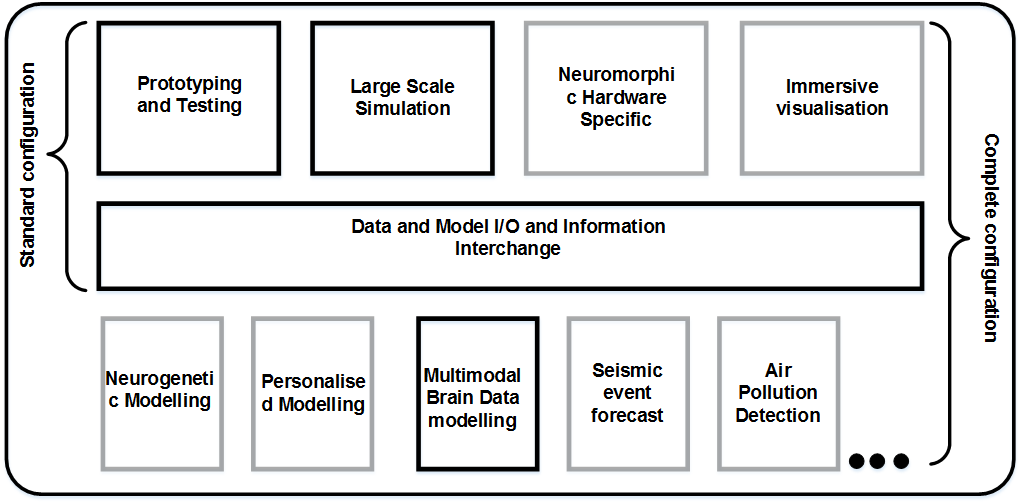
\includegraphics[width=\linewidth]{fig/neucube/neucube_multimodular.png}
	\caption{Block diagram of the multi-modular NeuCube software architecture.}
	\label{fig:neucube_multimodular}
\end{figure}

Any theoretical and conceptual design of pattern recognition system is invariably followed by implementation and design considerations. The design considerations necessary for applying the generalised NeuCube architecture in an application specific manner is well elaborated in \citep{scott2015thesis} and provides an useful insight on how to use \emph{a priori} knowledge in designing the NeuCube architecture. The multi-modular and rather minimally-constrained description of the NeuCube framework allows high flexibility in plugging in variety of algorithms and innovations as part of the framework. This flexibility also poses a great challenge in defining a clear ground truth of singularity in NeuCube. The evolution of NeuCube from a tool to perform neuro-informatic data analysis to a general purpose pattern recognition machine has also constrained the software development process to be unified in a single direction. \figurename \ref{fig:neucube_multimodular} introduces a block level diagram of the NeuCube software implementation strategy. This thesis directly contributes towards the development of the blocks highlighted in black. This architecture uses the core pattern recognition framework described earlier as the core component, and wraps a set of functionalities around the framework. There are three configuration abstractions present in the implementation strategy:

\begin{itemize}
	\item Basic configuration: The basic configuration includes a prototyping and testing module integrated with the I/O module. The main intention of this configuration is to use the NeuCube framework for general purpose pattern recognition, prototype model development and experimentation. Apart from model development capabilities, this module possesses additional integrated capabilities, such as dynamic visualisation, knowledge discovery and model analysis, and parameter optimisation modules. Due to the requirement of general purpose usage, this implementation is focused more towards usability and hence graphical user interface driven. The basic configuration is developed using Matlab and is freely available (licensed) for public usage. I will describe the design of the prototyping and testing software later in this Chapter.
	
	\item Standard configuration: The standard configuration is an extension of the basic configuration and includes development of scalable software for large scale experiments, and general purpose and neuromorphic hardware implementations. Since the prime focus is on scalability, the software implementations for large scale simulation are API driven and much more consideration is given to efficiency of implementation rather than usability. Additionally, the standard configuration also includes immersive visualisation of the NeuCube model for deeper analysis and knowledge discovery. These implementations generally follow strict software patterns and uses higher level languages like Java and Python. The contribution of this thesis towards the large scale implementation and simulation is presented in Chapter \ref{chap:large_snn}. 
	
	\begin{figure}
		\centering
		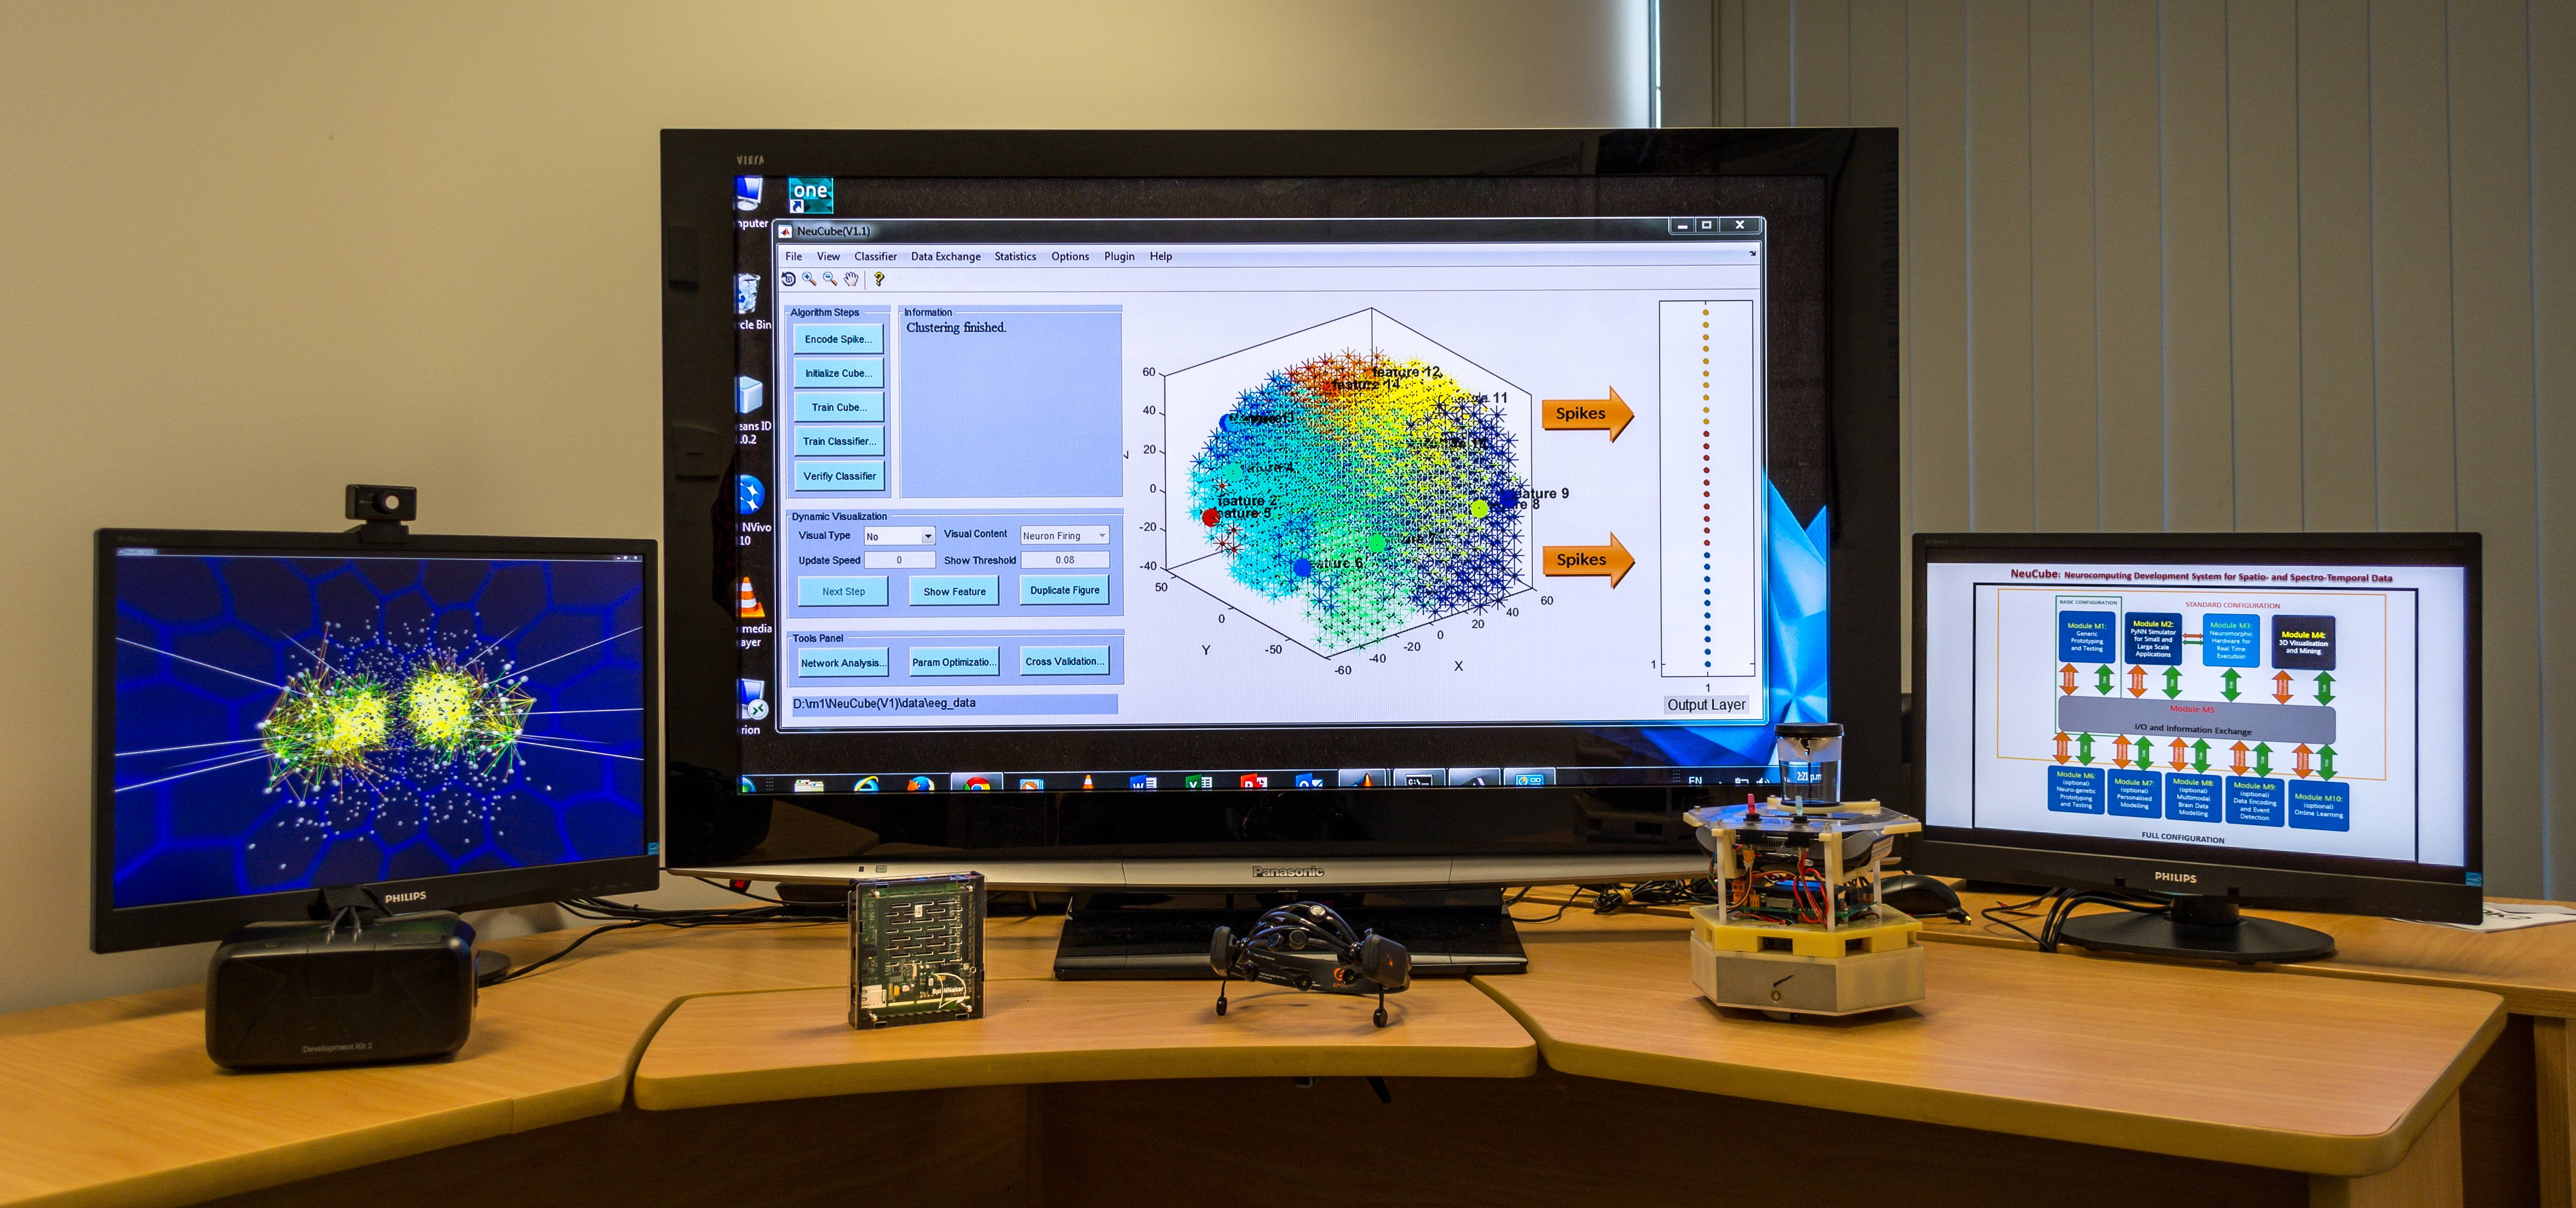
\includegraphics[width=\linewidth]{fig/neucube/neucube_standard.jpg}
		\caption{Standard configuration of the NeuCube software architecture consisting of the prototyping and testing module, immersive visualisation module and the SpiNNaker neuromorphic hardware chip.}
		
	\end{figure} 
	\item Full configuration: In addition to standard configuration, the full configuration includes all the application specific implementations of the NeuCube, such as personalised modelling, multi-modal brain data modelling, seismic event forecasting and so on. These application specific modules are developed for specific application purpose and extends the NeuCube architecture by adding application specific algorithms or functionality. This thesis contributes towards the development of methods and functionalities for multi-modal brain data. Chapters \ref{chap:encoding} and \ref{chap:multimodal} are dedicated to this topic.  
\end{itemize}

\subsection{NeuCube for Generic Prototyping and Testing of Applications}
The generic prototyping and testing tool is a GUI based Matlab implementation for rapid development of SNN application prototype systems for temporal or SSTD. The software is implemented as a set of continuous signal processing steps as shown in \figurename \ref{fig:neucube_archit}. The user interface of NeuCube, as shown in \figurename \ref{fig:neucube_ui}, is built as a set of functional components. An exhaustive description of the components can be found in the manual distributed along with the software. Here, I will briefly describe some of them:
\begin{figure}
	\centering
	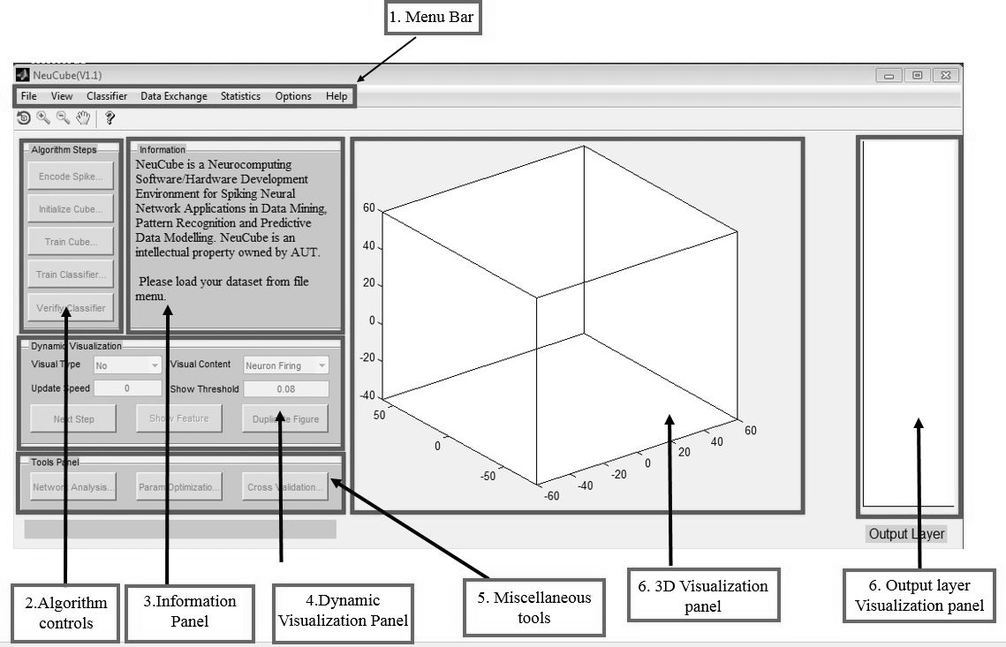
\includegraphics[width=\linewidth]{fig/neucube/ui.png}
	\caption{NeuCube generic prototyping and testing software user interface and panel descriptions.}
	\label{fig:neucube_ui}
\end{figure}

\subsubsection{I/O and Information Exchange}
  
The information exchange component is used to import or export user defined information to and from the software, which includes temporal or SSTD data, NeuCube models, parameters and results. This module interacts with the external environment using four data descriptors. They are the following:

\begin{itemize}
	\item Dataset descriptor: The Dataset descriptor consists of the data (and the meta data), that is to be learned and analysed. In the majority of cases, a dataset consists of a set of time series samples and the output label/value for the sample set. It is also possible to add miscellaneous information like ‘feature name’, ‘encoding method’ and other meta information in the dataset.
	\item SNNc descriptor: The SNNc descriptor is essentially the model descriptor containing all information related to the structure and learning of the SNN. Some of the most important information stored in this descriptor are the spatial information of the input and reservoir neurons, structural information of the SNNc and the state of the SNNc during learning.
	\item Parameter descriptor: The parameter descriptor stores all the user defined parameters including hyperparameters of data encoding algorithms, the unsupervised learning algorithm and the supervised learning algorithm.
	\item Result descriptor: The result descriptor stores information about the experimental results produced by NeuCube.
\end{itemize}
 
\begin{table}
	\centering
	\caption{Supported file format for descriptors.}
	\label{tab:descriptors}
	\begin{tabular}{@{}cccc@{}}
		\toprule \toprule
		Descriptor type & Mat & JSON & CSV \\ \midrule
		
		Dataset         & \cmark & \cmark  & \cmark \\
		SNNc            & \cmark & \cmark  & \xmark  \\
		Parameter       & \cmark & \cmark  & \xmark  \\
		Result          & \cmark & \xmark   & \cmark \\
		\bottomrule \bottomrule
	\end{tabular}
\end{table}

This module supports three different file formats, Mat (binary), JSON (structured text) and CSV (comma separated plain text). \tablename \ref{tab:descriptors} describes the supported file formats for each of the descriptor type.  As a heuristic, the Mat format is recommended for achieving faster I/O. The CSV files are the recommended choice for import/export of dataset and results for later analysis. The JSON format is recommended for inter modular communication. 

\subsubsection{Algorithm Interactions}

\begin{figure}
	\centering
	\subfloat[data encoding.]{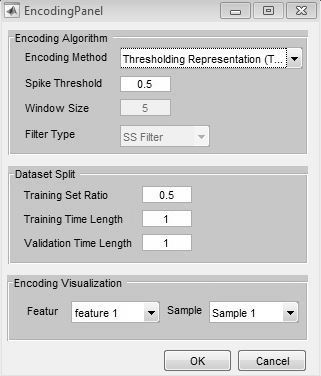
\includegraphics[width=0.4\linewidth]{fig/neucube/encoding_panel.png}%
		\label{fig:encoding_panel}}
	\hfil
	\centering
	\subfloat[SNNcube initialisation.]{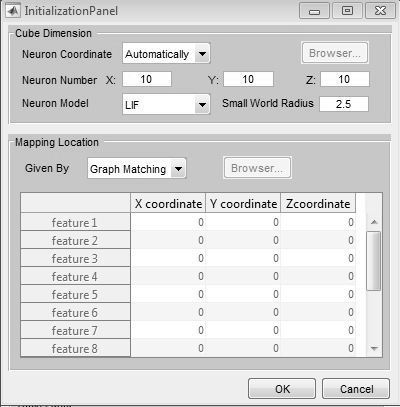
\includegraphics[width=0.4\linewidth]{fig/neucube/init_panel.png}%
		\label{fig:init_panel}}
	\hfil
	\centering
	\subfloat[Unsupervised learning.]{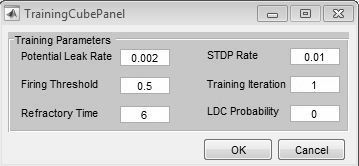
\includegraphics[width=0.4\linewidth]{fig/neucube/unsup_panel.png}%
		\label{fig:unsup_panel}}
	\hfil
	\centering
	\subfloat[Supervised learning.]{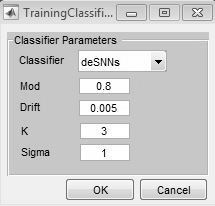
\includegraphics[width=0.4\linewidth]{fig/neucube/sup_panel.png}%
		\label{fig:sup_panel}}
	\caption{Algorithmic control UI panels.}
\end{figure}
This module allow users to interact with the pattern recognition and signal processing algorithms via the ’algorithm controls’ panel, shown in \figurename \ref{fig:neucube_ui}. The ’algorithm control’ panel includes a set of buttons for configuring and running the step by step process of data encoding, network initialisation, unsupervised learning (by training the SNNc) and supervised learning. The software uses a ’guided approach’ for performing the algorithmic steps by enabling or disabling buttons after every operation. \figurenames \ref{fig:encoding_panel}, \ref{fig:init_panel}, \ref{fig:unsup_panel} and \ref{fig:sup_panel} shows the individual user interaction panels for encoding, initialisation, unsupervised and supervised learning respectively. Each panel allows users to choose from a set of algorithms and corresponding hyperparameters. For example, the data encoding panel (\figurename \ref{fig:encoding_panel}) that encodes the real-valued signal to spike trains also provides the option of choosing from a set of encoding algorithms and it’s hyperparameters from the drop down menu. The algorithmic control interacts with the visualisation panels, for visualisation and analysis of the data and the models. 

\subsubsection{Integrated Visualisation and Network Analysis}
\label{subsec:vis}
Visualisation and model analysis is an integral feature of this module. Due to NeuCube's ability to create an interpretable and analysable model, the visualisation and analysis features plays an important part. Visualisation capabilities includes: comparative display of real and encoded data; online dynamic visualisation of the SNNc learning; Visualisation of the SNNc model and the output readout layer.

Analysis of an SNNc network can be performed using the network analysis toolbox. This toolbox includes a bunch of graph analysis capabilities for measuring and visualising interactions between nodes and edges the SNNc at different levels. The network analysis consists of two major functionalities: (1) Neuron cluster analysis; and, (2) Information route analysis. An example of neuron cluster analysis is shown in \figurename \ref{fig:cluster_analysis} 

\begin{figure}
	\centering
	\subfloat{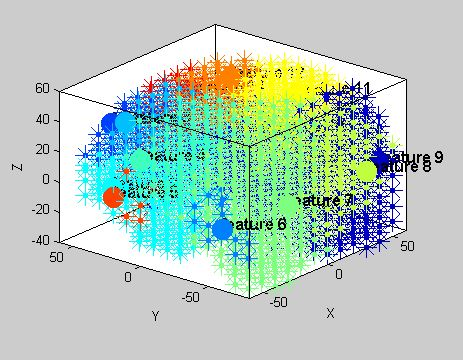
\includegraphics[width=0.45\linewidth]{fig/neucube/cluster_analysis.JPG}%
	}
	\hfil
	\centering
	\subfloat{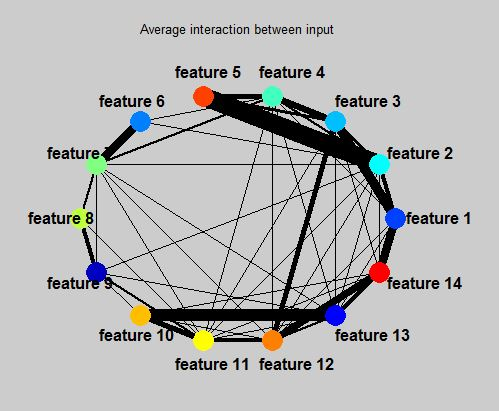
\includegraphics[width=0.45\linewidth]{fig/neucube/average_interaction.JPG}%
	}
	\caption{Neuron cluster analysis by network analysis toolbox (A)Neuron clustering based on connection weights of the network (B)average one to one interaction between the input nodes. The thicker lines signifies more interaction.}
	\label{fig:cluster_analysis}
\end{figure}

\paragraph{Parameter optimisation}

Parameter optimisation is developed to allow users to search for the optimal set of hyperparameters for the NeuCube prototype system (model). The computational time for parameter optimisation depends on the number of parameters to be optimised and the size of the NeuCube model. Parameter optimisation, can be performed using various methods, such as: Grid search; Genetic Algorithm; Differential Evolution; Quantum Inspired Evolutionary Algorithms, and PSO. The current release of NeuCube includes two methods (Grid search and Genetic algorithm).


\subsection{NeuCube Based Spatio-temporal Data Research and Applications}
\label{sec:app}
\subsubsection{Application of NeuCube in Brain Data Modelling}

A number of recent studies have applied NeuCube architecture to brain data modelling, especially using ElectroEncephalography (EEG) data and functional Magnetic Resonance Images (fMRI) brain data. The spatio-temporal information contained in EEG and fMRI data poses challenges to standard statistical or machine learning techniques. Though, often standard machine learning techniques are used to process spatio-temporal brain data, they lack the ability: (1) to recognise differences in neurological dynamics that occur over the time; (2) identify the functional brain area involved; and, (3) to quantify the information involved. The RNN architecture of NeuCube, however, improves such capabilities \citep{taylor2014feasibility, hu2014eeg, kasabov2013dynamic}. In \citep{capecci2015analysis} for example, NeuCube was used to study mental tasks using data collected by a 19-channel EEG recorder. This research showed the ability of NeuCube to classify and analyse changes in functional brain activities. This study was quite significant for identification of the appearance of mild cognitive impairment (MCI) and the staging of its degeneration toward Alzheimer’s Disease (AD). Recently, there has been a huge interest in using functional magnetic resonance imaging (fMRI) to understand, analyse and predict behaviour and cognition. The ability of fMRI to sample high resolution spatial information over time has been successfully used in correlating high resolution neural activity with behaviour. NeuCube has been used in several studies \citep{doborjeh2014classification, kasabov2017mapping} involving fMRI data. 

\subsubsection{NeuCube for BCI}
The feasibility of using NeuCube with EEG data to develop a functional electrical stimulation BCI/BMI system that is able to assist in the rehabilitation of complex upper limb movements was shown in \citep{taylor2014feasibility}. In order to provide an effective tool for this purpose, a NeuCube model was trained on EEG data for a series of relatively complex muscle movements. The preliminary experiments suggest that NeuCube is much more efficient for this task than standard machine learning techniques, resulting in high recognition accuracy, a better adaptability to new data, and a better interpretation of the models, leading to a better understanding of the brain data and the processes that generated it.

\subsubsection{NeuCube for Neuro-rehabilitation}

Neuro-rehabilitation is another area of research NeuCube was applied as feasibility analysis study. Biomimetic learning and information processing time-scales of NeuCube provides appropriate technology for integration with mental tasks. In addition, the fast and incremental learning offered by the framework is capable of adapting to the users' changing abilities as their rehabilitation progresses. Repetitive activities of daily living (ADL) and robotic active training are commonly practised in the rehabilitation of paralysed patients, both of which have been proven effective in the recovery of locomotor function in impaired limbs. Classification of ADL from EEG is of interest for the active robotic rehabilitation of patients with spinal cord injuries (SCI). This classification is a significant challenge with classical techniques, as these cannot manage the high noise, variability, and gradual change (due to the subject learning or rehabilitating the task) in the EEG signals effectively. \citet{hu2014eeg} performed an experiment using the NeuCube eSTDM to identify the upper-limb ADL of three classes with 14-channel EEG data. Classification accuracy using this technique is shown to be promising despite the highly noisy, low resolution EEG data \citep{hu2014eeg}. This experiment indicates strong potential for further exploration of the  NeuCube for neuro-rehabilitation tasks.

\subsubsection{NeuCube for SSTD Modelling in Other Applications}
Several applications of NeuCube in the above areas are described in \citep{kasabov2016evolving, doborjeh2018from}, including: individual risk of stroke prediction based on personal, static data and temporal climate data; early experimental results on earthquake prediction; predicting establishment of harmful species in ecology; and stock index prediction.




\pagebreak
\section{Contributions and Publications}
\begin{tcolorbox}[colback=black!5,colframe=black!40!black,title=Contributions]
	\itshape
	\begin{enumerate}
		\item Introduction to recurrent neural networks and evolution of reservoir computing and liquid state machines.
		\item Overview of the NeuCube evolving spatio-temporal data machine architecture.
		\item Description of the Software design framework of NeuCube and the NeuCube prototyping and testing environment. 
	\end{enumerate}
\end{tcolorbox}

\begin{tcolorbox}[colback=black!5,colframe=black!40!black,title=Publications]
	\begin{enumerate}
		\item Kasabov, N., Scott, N. M., Tu, E., Marks, S., \textbf{Sengupta, N.}, Capecci, E., ... \& Espinosa-Ramos, J. I. (2016). Evolving spatio-temporal data machines based on the NeuCube neuromorphic framework: design methodology and selected applications. Neural Networks, 78, 1-14.
		\item \textbf{Sengupta, N.}, Ramos, J.I.E., Tu, E., Marks, S., Scott, N.,... \& Abbott, A. (2018). From von Neumann architecture and Atanasoffs ABC to Neuromorphic Computation and Kasabov’s NeuCube: Principles and Implementations, Learning Sytems: From Theory to Practice Springer.
	\end{enumerate}
\end{tcolorbox}
